\section{Teoria do Git}

\begin{frame}{O que são commits?}
  \centering
  \only<1>{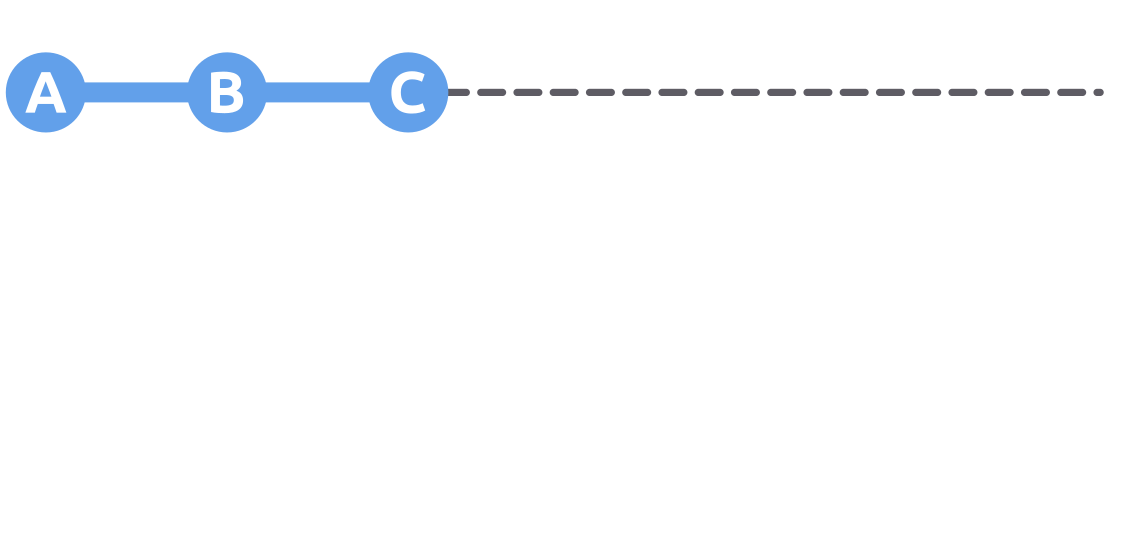
\includegraphics[width=1\linewidth]{git-commit1.png}}
  \only<2>{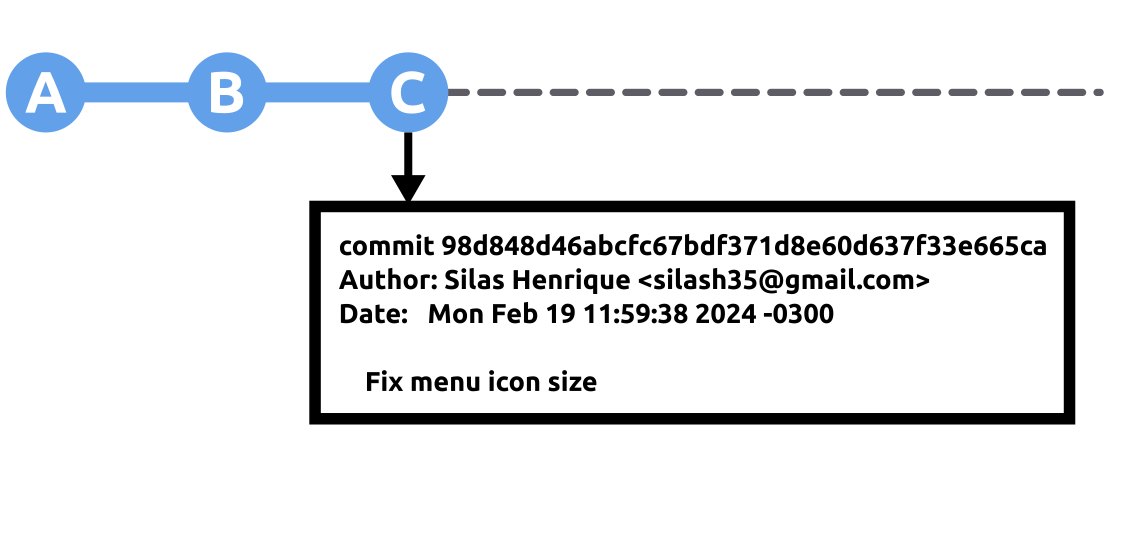
\includegraphics[width=1\linewidth]{git-commit2.png}}
\end{frame}

\note{
  Um commit é um registro de uma alteração no histórico do projeto.
  Ele representa um estado do projeto naquele momento e guarda informações como quem fez a alteração, quando ela foi feita e uma mensagem descrevendo o que foi alterado.
  Todo commit também possui um identificador único.
  Esse identificador permite referenciar exatamente aquele commit no histórico do projeto.

  Tá vendo? Só isso. Bem simples.

  E aí, conforme criamos commits, essas relações começam a formar uma estrutura de grafo.

  Mais especificamente, o histórico de commits do Git forma um grafo acíclico direcionado: cada commit aponta para um ou mais commits anteriores.

  Quem achou que não ia utilizar estrutura de dados para nada?
}

\begin{frame}{O fluxo de trabalho do Git}
  \centering
  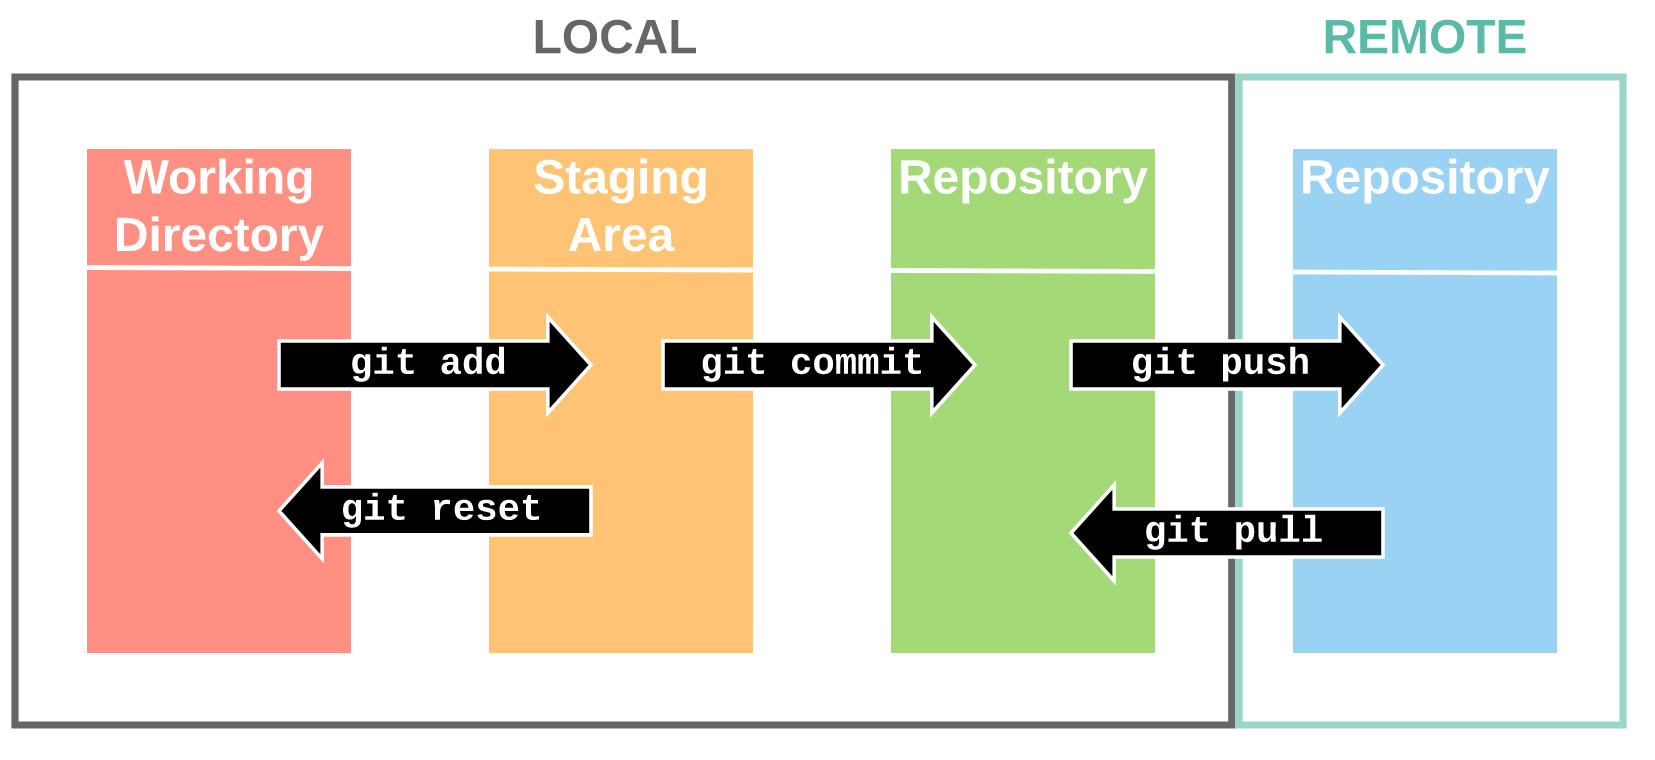
\includegraphics[width=1\linewidth]{git-workflow.jpg}
\end{frame}

\note{
  Vamos imaginar que estamos trabalhando em um projeto.

  Primeiro, estamos simplesmente editando os arquivos.
  Esse é o Working Directory: o estado atual dos arquivos no nosso computador.

  Agora fizemos três alterações: corrigimos um erro, adicionamos uma funcionalidade e também alteramos a documentação.
  Mas talvez não queiramos registrar as três coisas juntas no mesmo commit.
  Queremos fazer um commit apenas com a correção do erro.

  É aí que entra a Staging Area.
  Ela funciona como uma área de preparação: colocamos nela exatamente as alterações que queremos incluir no próximo commit.

  Quando fazemos o commit, essas alterações passam a fazer parte do histórico do nosso Local Repository.
  Esse histórico fica no nosso computador e podemos consultá-lo sem precisar de internet.
}

\note{
  Depois, quando quisermos compartilhar esses commits, enviamos nosso histórico para um Remote Repository.
  Esse tal de Remote Repository pode ser o GitHub, o GitLab ou qualquer outra plataforma que você estiver utilizando.

  Mas ele nem precisa estar na internet.
  Pode ser simplesmente outro repositório em outra máquina ou até outra pasta no seu próprio computador.
  O Git não sabe nem se importa se existe um GitHub por trás disso.
}